\documentclass[10pt,twocolumn,letterpaper]{article}

\usepackage{cvpr}
\usepackage{times}
\usepackage{epsfig}
\usepackage{graphicx}
\usepackage{amsmath}
\usepackage{amssymb}
\usepackage{bm}
\usepackage{overpic}
\usepackage{multirow}
\usepackage{booktabs}       % professional-quality tables
\usepackage{array}

% Include other packages here, before hyperref.

% If you comment hyperref and then uncomment it, you should delete
% egpaper.aux before re-running latex.  (Or just hit 'q' on the first latex
% run, let it finish, and you should be clear).
\usepackage[pagebackref=true,breaklinks=true,letterpaper=true,colorlinks,bookmarks=false]{hyperref}

\cvprfinalcopy % *** Uncomment this line for the final submission

\def\cvprPaperID{1251} % *** Enter the CVPR Paper ID here
\def\httilde{\mbox{\tt\raisebox{-.5ex}{\symbol{126}}}}
\def\blu#1{\textbf{\color{blue} #1}} %in Table

% Pages are numbered in submission mode, and unnumbered in camera-ready
\ifcvprfinal\pagestyle{empty}\fi
\begin{document}

%%%%%%%%% TITLE
\title{PiCANet: Learning Pixel-wise Contextual Attention for Saliency Detection\\
Supplemental Material}

\author{
	Nian Liu$^{1}$
	\hspace{25pt}
	Junwei Han$^{1}$
	\hspace{25pt}
	Ming-Hsuan Yang$^{2,3}$
	\\
	$^1$Northwestern Polytechincal University
	\hspace{8pt}
	$^2$University of California, Merced
	\hspace{8pt}
	$^3$Google Cloud
	\\
	{\tt\small
    \{liunian228, junweihan2010\}@gmail.com
    \hspace{50pt}
    mhyang@ucmerced.edu
    }
}

\maketitle
\thispagestyle{empty}

In this supplementary material, we include more implementation details, more ablation analyses, and more experimental results.

%%%%%%%%% BODY TEXT
\section{Additional Implementation Details}

\subsection{Using the ResNet50 Backbone}

When using the ResNet50 network \cite{he2016resnet} as the backbone, we modify the $4^{th}$ and the $5^{th}$ residual blocks to have strides of 1 and dilations of 2 and 4, respectively, thus making the encoder have a stride of 8. Then we progressively fuse the feature maps from the $5^{th}$ to the $1^{st}$ Conv blocks in the decoding modules $\mathcal D^5$ to $\mathcal D^1$. We adopt global PiCANets in $\mathcal D^5$ and $\mathcal D^4$, and local PiCANets in the last three modules, respectively. In each decoding module $\mathcal D^i$, we use the final Conv feature map of the $i^{th}$ Conv block in the ResNet50 encoder (\eg res4f and res3d) as the incorporated encoder feature map $\bm{En}^i$ and do not adopt the BN and the ReLU layers on it as shown in Figure 3(b) since the ResNet50 network has already used BN layers after each Conv layer. The final generated saliency map is of size $112\times 112$ since the conv1 layer has a stride of 2.

As the same as when using the VGG-16 backbone, we empirically set the loss weights in $\mathcal D^5,\mathcal D^4,\cdots,\mathcal D^1$ as 0.5, 0.5, 0.8, 0.8, and 1, respectively. The minibatch size of our ResNet50 based network is set to 8 due to the GPU memory limitation. The other hyperparameters are set as the same as the ones used in the VGG-16 based network. The testing time for one image is 0.236s.

\subsection{Using the CRF Post-processing}

When we adopt the CRF post-processing method, we use the same parameters and the same code used by \cite{hou2017dss}. It additionally costs another 0.09s for each image.


\section{Experiments}

\subsection{Effectiveness of Progressively Embedding PiCANets}

\begin{table} [!t]
\begin{center}
\caption{Effectiveness of progressively embedding PiCANets. ``+75G432LP'' means using \textbf{G}lobal PiCANets in $\mathcal D^7$ and $\mathcal D^5$, and \textbf{L}ocal \textbf{P}iCANets in $\mathcal D^4$, $\mathcal D^3$, $\mathcal D^2$. Other settings can be inferred similarly. \blu{Blue} indicates the best performance.}
\vspace{1mm}
\label{progressiveTab}
\footnotesize
\begin{tabular}{@{}lccccccc@{}}
\toprule
\multirow{2}{*}{Settings} & \multicolumn{3}{c}{DUT-O \cite{yang2013gbmr}}  && \multicolumn{3}{c}{DUTS-TE \cite{wang2017duts}} \\
\cmidrule{2-4} \cmidrule{6-8}
                          &  $F_{\beta}$   &  $F_{\beta}^{\omega}$  &   MAE    && $F_{\beta}$   &  $F_{\beta}^{\omega}$  &   MAE  \\ \midrule
U-Net \cite{ronneberger2015unet} & 0.761   & 0.651                  & 0.073    && 0.819         & 0.715                  & 0.060  \\ \midrule
+7GP                      & 0.772          & 0.660                  & 0.071    && 0.826         & 0.722                  & 0.058  \\
+75GP                     & 0.778          & 0.662                  & 0.071    && 0.834         & 0.724                  & 0.057  \\
+75G4LP                   & 0.785          & 0.678                  & 0.069    && 0.840         & 0.736                  & 0.056  \\
+75G43LP                  & 0.791          & 0.682                  &\blu{0.068}&& 0.848        & 0.740                  & 0.055  \\
+75G432LP                 &\blu{0.794}     &\blu{0.691}             &\blu{0.068}&&\blu{0.851}   &\blu{0.748}             &\blu{0.054}\\
\bottomrule
\end{tabular}
\vspace{-0.7cm}
\end{center}{}
\end{table}

Here we report a more detailed ablation study of progressively embedding PiCANets in each decoding module. As shown in Table~\ref{progressiveTab}, progressively embedding global and local PiCANets in $\mathcal D^7,\mathcal D^5,\mathcal D^4,\cdots,\mathcal D^1$ can consistently improve the saliency detection performance, thus demonstrating the effectiveness of our proposed PiCANets and the saliency detection model.

\subsection{More Visualization of the Learned Attention Maps}

\begin{figure*}[!t]
  \graphicspath{{Figures/attention/}}
  \centering
  %\begin{overpic}[width=1\linewidth,grid,tics=2]{attention_sup.jpg}
  \begin{overpic}[width=1\linewidth]{attention_sup.jpg}
  \put(2,1){\small Image/GT/SM}
  \put(21,1){\small att($\mathcal D^7$)}
  \put(37,1){\small att($\mathcal D^5$)}
  \put(53,1){\small att($\mathcal D^4$)}
  \put(69,1){\small att($\mathcal D^3$)}
  \put(85,1){\small att($\mathcal D^2$)}
  \end{overpic}
  \caption{Illustration of the learned attention maps of the proposed PiCANets. The first column shows two images and their corresponding ground truth masks and the predicted saliency maps of our model while the last five columns show the attention maps in five attended decoding modules, respectively. For each image, we give three example pixels (denoted as red dots. The first row shows a background pixel and the bottom two rows show two foreground pixels). The attended context regions are marked by red rectangles.}
  \label{attention_sup}
  \vspace{-0.4cm}
\end{figure*}

We illustrate more learned attention maps in Figure~\ref{attention_sup} for the five attended decoding modules. Figure~\ref{attention_sup} shows that the global attention learned in $\mathcal D^7$ and $\mathcal D^5$ can attend to foreground objects for background pixels and backgrounds for foreground pixels. The local attention learned in $\mathcal D^4$, $\mathcal D^3$, and $\mathcal D^2$ can attend to regions with similar semantics with the referred pixel.

\subsection{More Visual Comparison Between Our Model and Stata-of-the-Art Methods}

\begin{figure*}[!t]
  \graphicspath{{Figures/qualitative/}}
  \centering
  %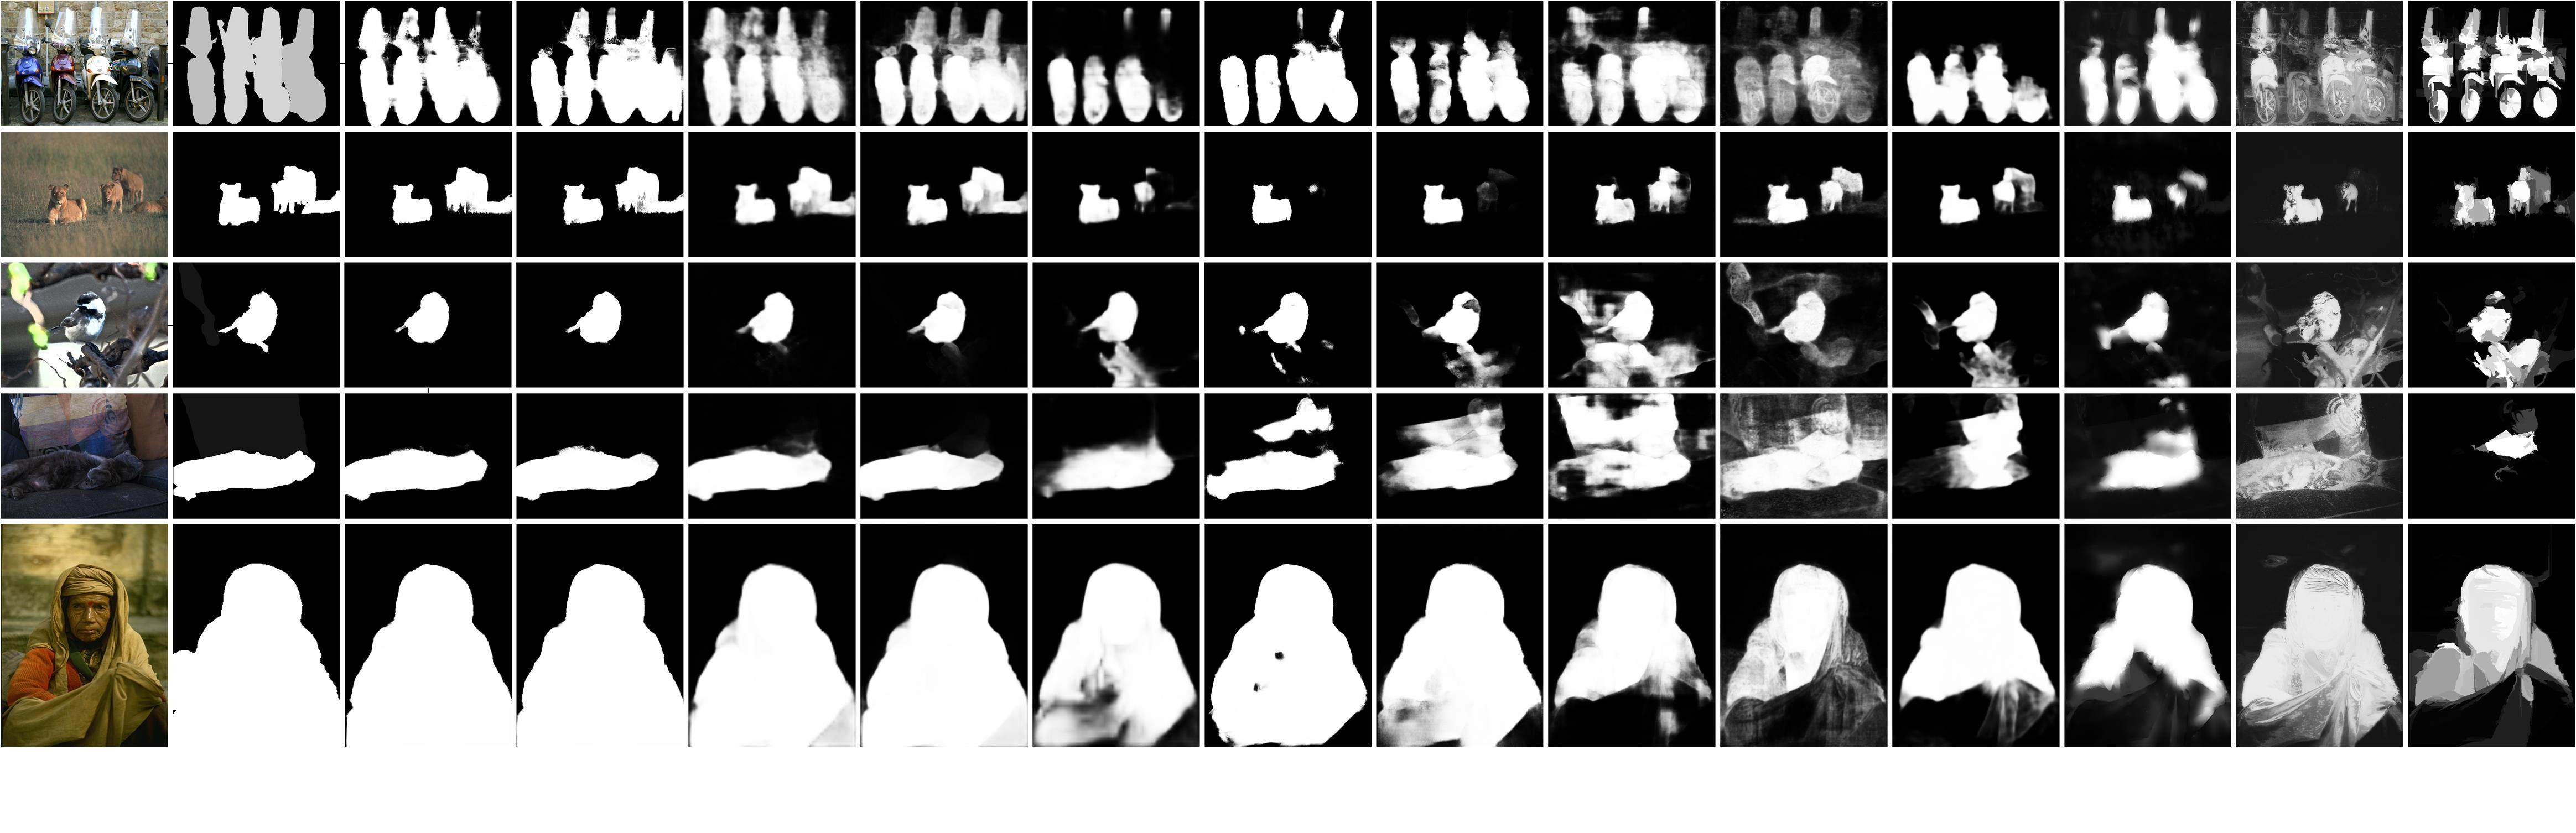
\includegraphics[width=1\linewidth]{qualitative.jpg}
  %\begin{overpic}[width=1\linewidth,grid,tics=1]{qualitative.jpg}
  \begin{overpic}[width=1\linewidth]{qualitative_sup.jpg}
  \put(1,1.5){\scriptsize Image}
  \put(9,1.5){\scriptsize GT}
  \put(13.8,0.5){\scriptsize \shortstack[c] {PiCANet\\ -RC}}
  \put(20.8,0.5){\scriptsize \shortstack[c] {PiCANet\\ -C}}
  \put(27.5,0.5){\scriptsize \shortstack[c] {PiCANet\\ -R}}
  \put(34.5,1.5){\scriptsize PiCANet}
  \put(40.5,1.5){\scriptsize SRM \cite{Wang2017srm}}
  \put(48,1.5){\scriptsize DSS \cite{hou2017dss}}
  \put(53.5,1.5){\scriptsize NLDF \cite{luo2017nldf}}
  \put(60,1.5){\scriptsize Amulet \cite{Zhang2017amulet}}
  \put(67.3,1.5){\scriptsize UCF \cite{Zhang2017ucf}}
  \put(74,1.5){\scriptsize DHS \cite{liu2016dhsnet}}
  \put(80.2,1.5){\scriptsize RFCN \cite{wang2016rfcn}}
  \put(87.6,1.5){\scriptsize DCL \cite{li2016dcl}}
  \put(94,1.5){\scriptsize MDF \cite{li2015mdf}}
  \end{overpic}
  \caption{Qualitative comparison. (GT: ground truth)}
  \label{visualcmp_sup}
  %\vspace{-0.3cm}
\end{figure*}

We also show more qualitative results in Figure~\ref{visualcmp_sup}. It shows that compared with other state-of-the-art methods, our model can highlight salient objects more accurately and uniformly under various challenging scenarios even without using post-processing techniques.

\subsection{Failure Cases}

\begin{figure*}[!t]
  \graphicspath{{Figures/failureCases/}}
  \centering
  %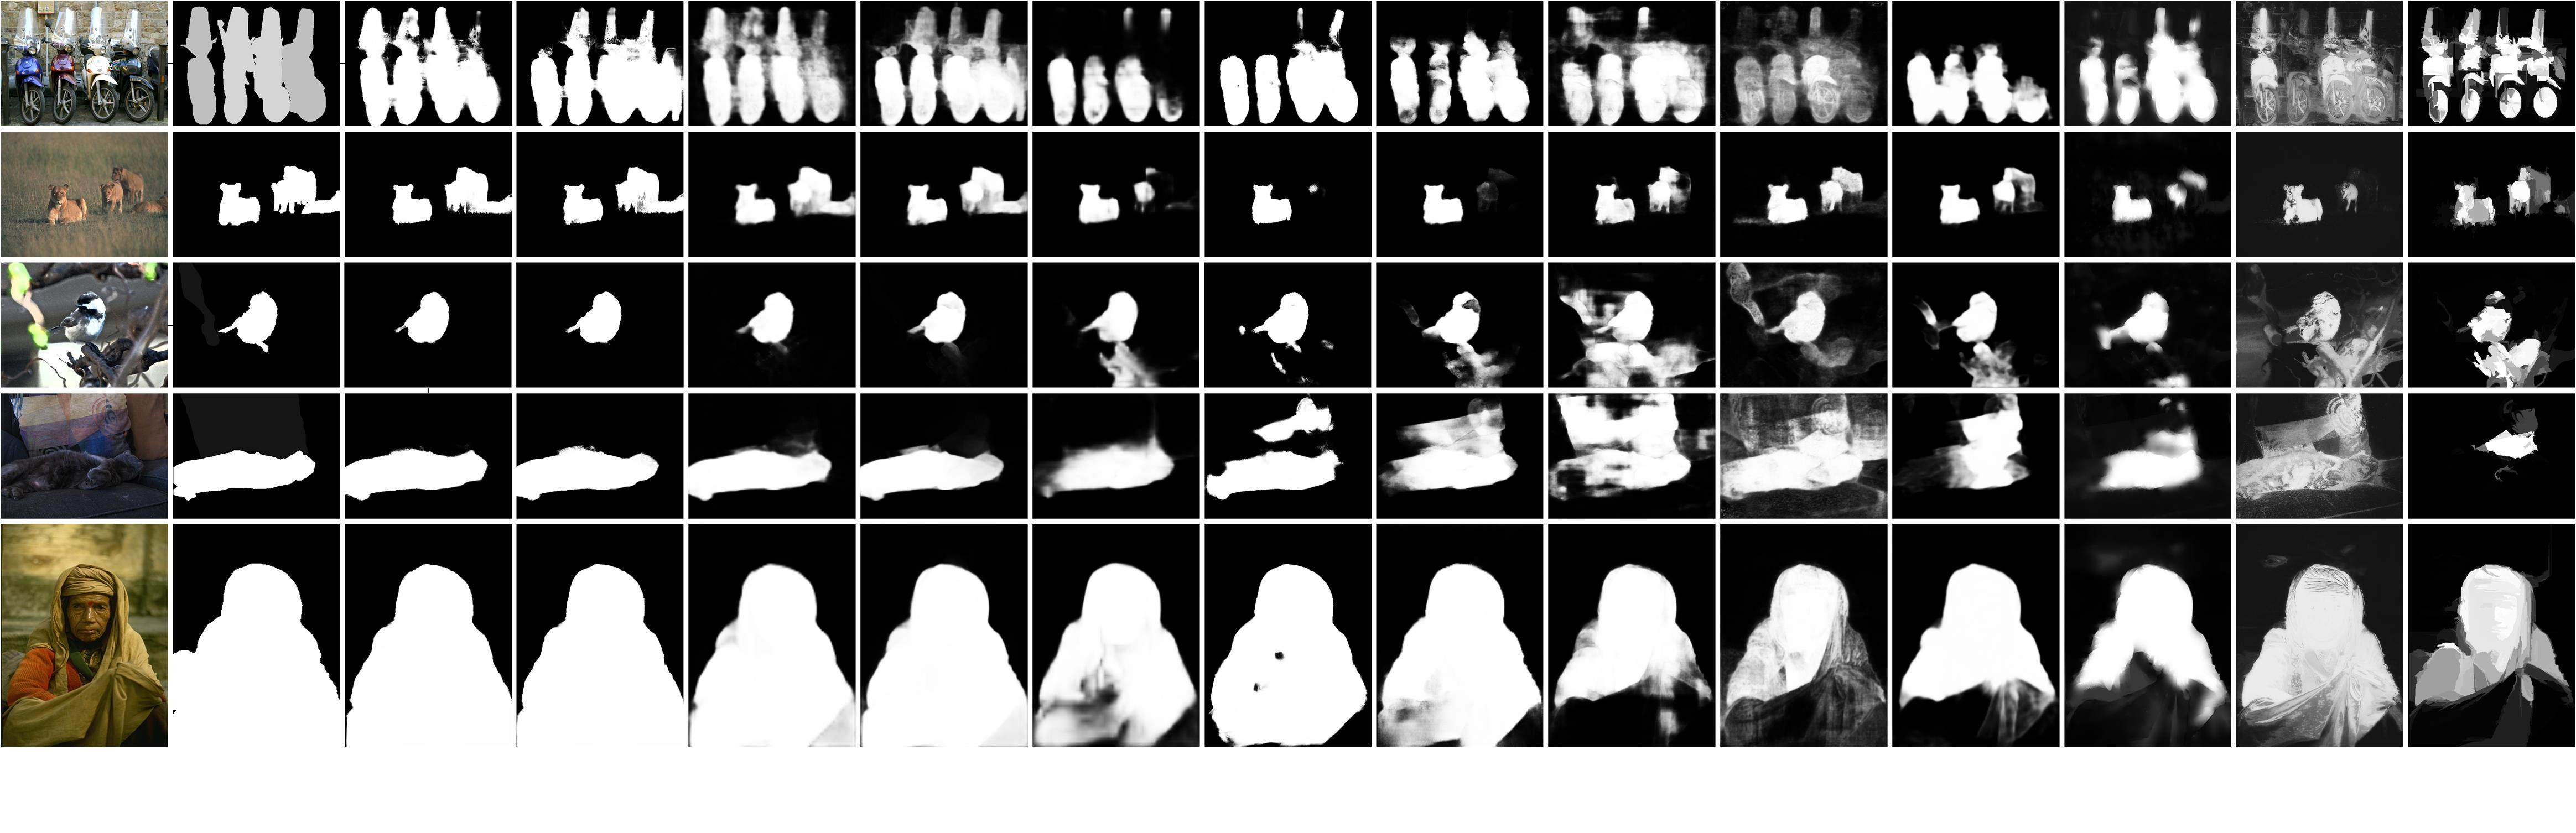
\includegraphics[width=1\linewidth]{qualitative.jpg}
  %\begin{overpic}[width=1\linewidth,grid,tics=1]{qualitative.jpg}
  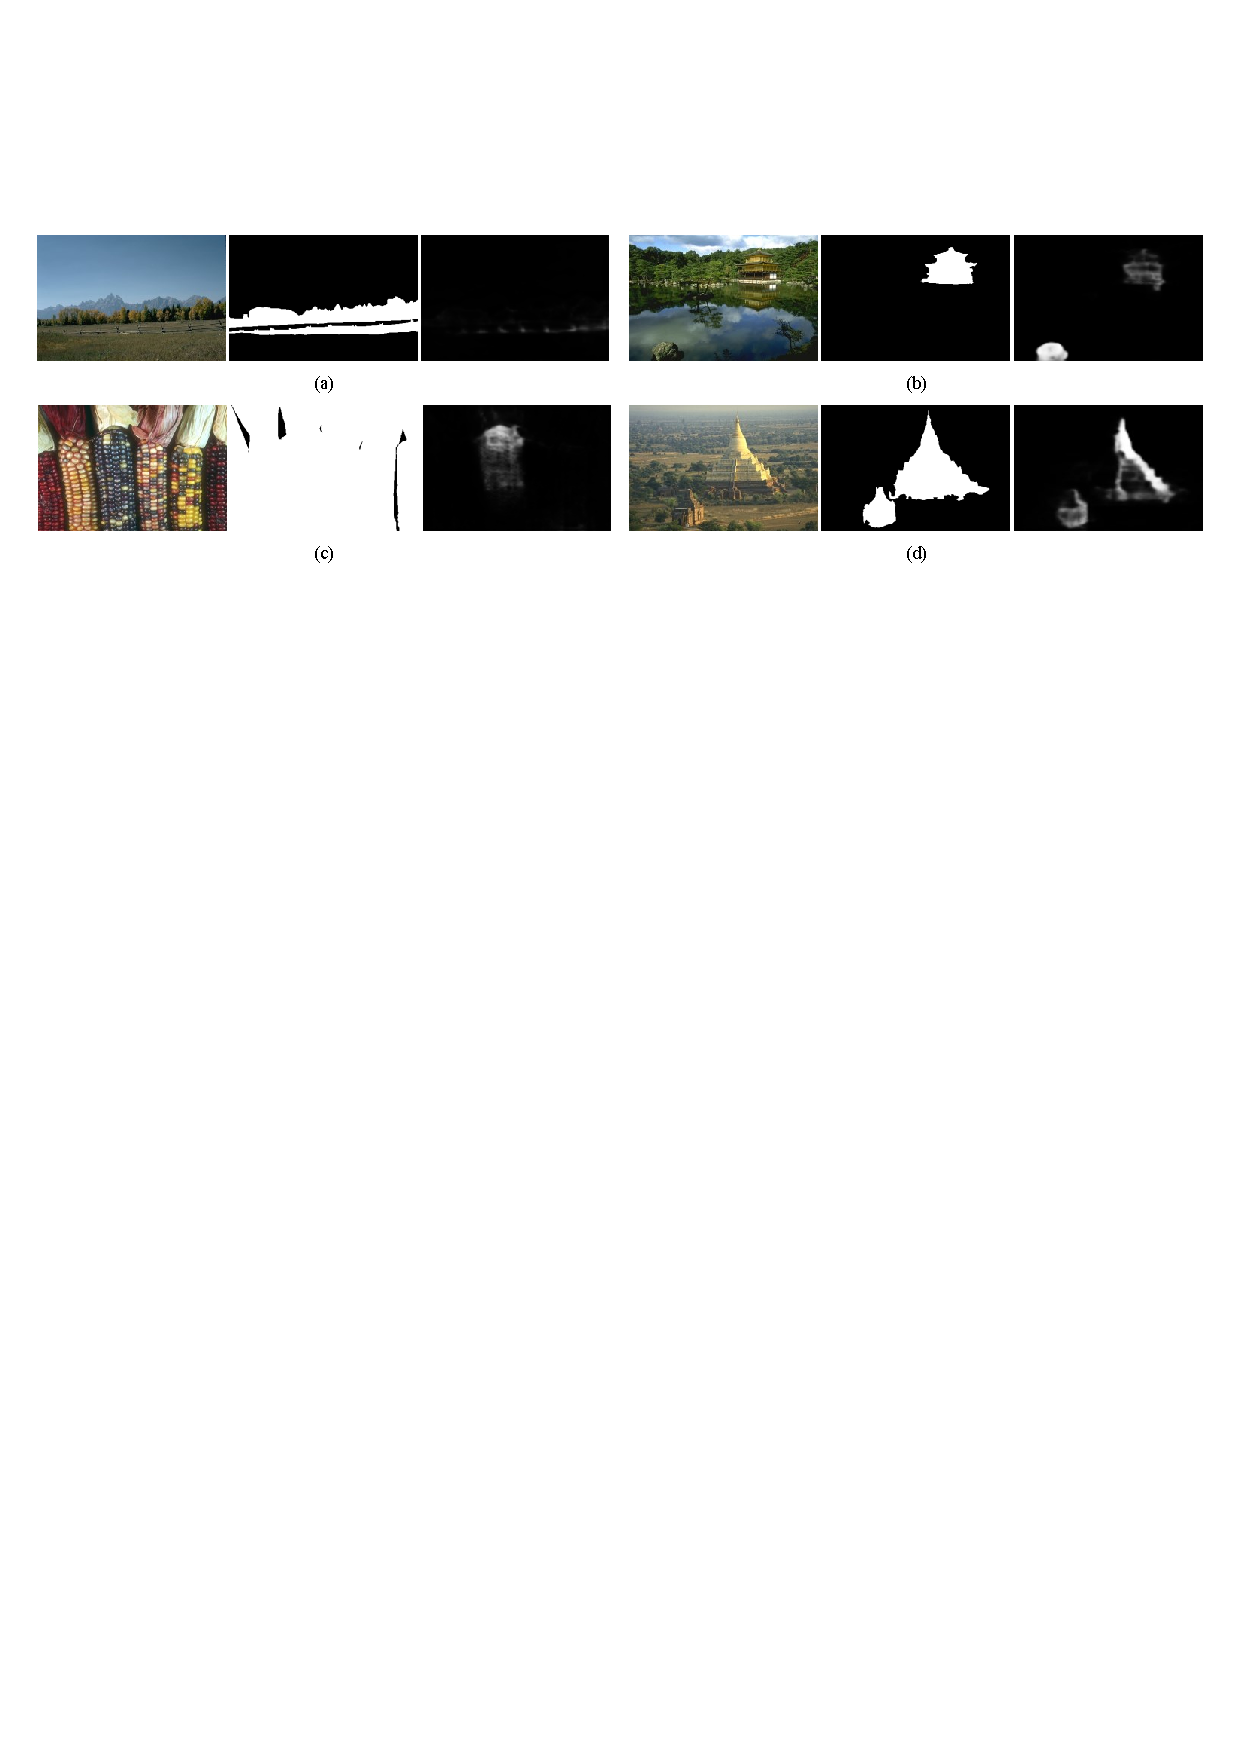
\includegraphics[width=1\linewidth]{failurecases.pdf}
  \caption{Failure cases. The three images in each set are the input image, the ground truth, and our result, respectively.}
  \label{failure_cases}
  \vspace{-0.3cm}
\end{figure*}

We show some failure cases of our PiCANet-R model in Figure~\ref{failure_cases}. Basically, our model usually fails when the image has no obvious foreground objects, as shown in (a) and (b). (c) shows that when the foreground object is extremely large, our model is also easy to fail. While these two situations are also challenging to other traditional and deep learning based saliency models, indicating that we still have much room to improve current models. (d) shows that the non-uniform illumination on the object may also mislead our model.

{\small
\bibliographystyle{ieee}
\bibliography{cvpr18_PiCANet_saliency}
}

\end{document}
